\chapter{Flow Solver With Automatic Differentiation}
\label{ch:FlowSolver}
To test Julia's AD tools in a real world application I have implemented an example taken from the MATLAB Reservoir Simulation Toolbox (MRST) and implemented it in Julia. MRST is primary developed by the Computational Geosciences group in the department of Mathematics and Cybernetics at SINTEF Digital \emph{\citep{mrstHomepage}}. According to MRST's homepage, "MRST is not primarily a simulator, but is mainly intended as a toolbox for rapid prototyping and demonstration of new simulation methods and modelling concepts." Although most of the tools and simulators in MRST are very efficient and perform well -- if you are to simulate more heavy simulation, they recommend to use the Open Porous Media (OPM) Flow simulator \emph{\citep{OPM}}. OPM is a toolbox to build simulations of porous media processes that are mainly written in C++ and C. Here, the differences between the languages become clear. As MATLAB with its easy to use mathematical syntax is a great language to quickly make prototypes and demonstrations of simulations, it is failing somewhat when it comes to computational speed. But where MATLAB fails in computational speed, C++ and C are two very fast languages. The problem with C++ and C is that these languages are not built for numerical analysis, hence it takes longer time to create the simulations. This is where Julia comes in. As the founders of Julia stated: Julia is meant to be a language as familiar as MATLAB in terms of mathematical notations, but as fast as C in terms of computational speed. Hence, it is interesting to figure out how Julia can perform compared to MRST.

To compare different AD implementations in Julia and MATLAB I have implemented MRST's tutorial, "Single-phase Compressible AD Solver" from \texttt{flowSolverTutorialAD.m} \emph{\citep{flowSolverADExample}}, in Julia. The example is made as an introduction to how AD can be used in MRST, hence it is a good example to use when the goal is to compare the implementation of AD in MATLAB and Julia. 

\section{Grid Construction}
The example consist of modelling how the pressure drops within a rectangular reservoir measuring $200\times 200 \times 50 \text{m}^3$ when we have a well that that is producing oil. "Single-phase solver" only means that we do not have different phases of fluid, like liquid and gas, present during the simulation. As the purpose of this example is to compare the AD tools in MATLAB and Julia and not the process of solving the problem, including setting up the grid and other necessary variables, some of the initialization and plotting have been performed in Julia by calling code from MRST. This has been done by using the package MATLAB.jl \emph{\citep{MATLAB.jl}}. This package allows calling MATLAB functions from Julia and retrieve the output variables. This is done by the function call
\lstinputlisting{code/mxcall.jl}
where we have three input parameter and two output parameters. We have to specify the number of output parameters after the MATLAB function name.  By calling MATLAB from Julia, we can use MRST's \texttt{G = computeGeometry(...)} function to set up the grid for the simulation. The grid of the reservoir can be seen in \autoref{fig:flowSolverGrid}. The variable \texttt{G} that contains the grid properties is now a structured array (struct), having all the information on cells, facets, vertices and nodes that we need to make the discrete divergence and gradient operators as explained in \autoref{sec:ApplicationsAD}. 

Next, we define the properties of the rock. In an oil reservoir, the oil lies inside porous rock and hence the properties of the rock will affect the flow of the oil. The amount of oil we can have inside the rock is measured as pore volume. First, we make a new variable \texttt{rock} that contains parameters that describe the rock's ability to store and trasmit fluids for each cell with the function \texttt{rock = makeRock(...)}. Then, we say that in our model the rock is compressed constantly as a function of pressure and we obtain the analytic solution for the pore volume as a function of pressure
\begin{equation}
    pv(p) = \text{pv}_r \exp[c_r\cdot(p-p_r)],
    \label{eq:poreVolume}
\end{equation}
where pv$_r$ is the rock pore volume properties, in a cell, at a reference pressure $p_r$. $c_r$ is a constant controlling how the rock is compressed. The pore volume of the rock as a function of pressure values are visualized in \autoref{fig:flowSolverPoreVolume}. The graph shows that for a cell with volume $1000\text{m}^3$ there is approximately room for $600\text{m}^3$ oil.

Since we assume that the oil have a constant compressibility, the density of the oil is given as an analytic function of pressure 
\begin{equation}
    \rho(p) = \rho_r\exp[c\cdot(p-p_r)],
    \label{eq:pressureSolverDensity}
\end{equation}
where $\rho_r = 850\text{kg}/\text{m}^3$ and $c$ is a constant controlling how fast the oil is compressed. The density of the fluid as a function of pressure is plotted for some pressure values in \autoref{fig:flowSolverDensity}.
\begin{figure}[H]
    \centering
    \begin{subfigure}[t]{0.48\textwidth}
        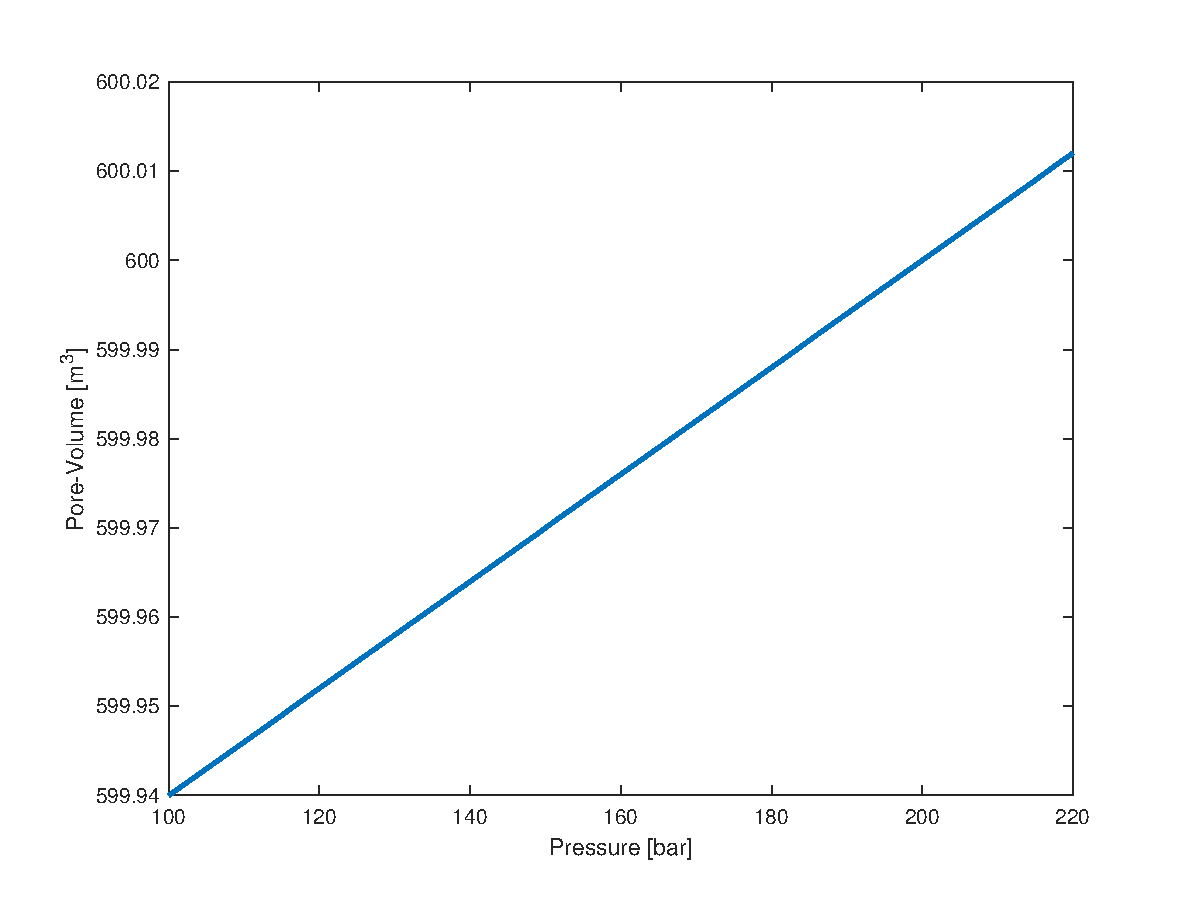
\includegraphics[width=\textwidth]{figures/flow_solver_pore-volume.eps}
        \caption{The pore volume of the rock in a cell as a function of pressure.}
        \label{fig:flowSolverDensity}
    \end{subfigure}
    \begin{subfigure}[t]{0.48\textwidth}
        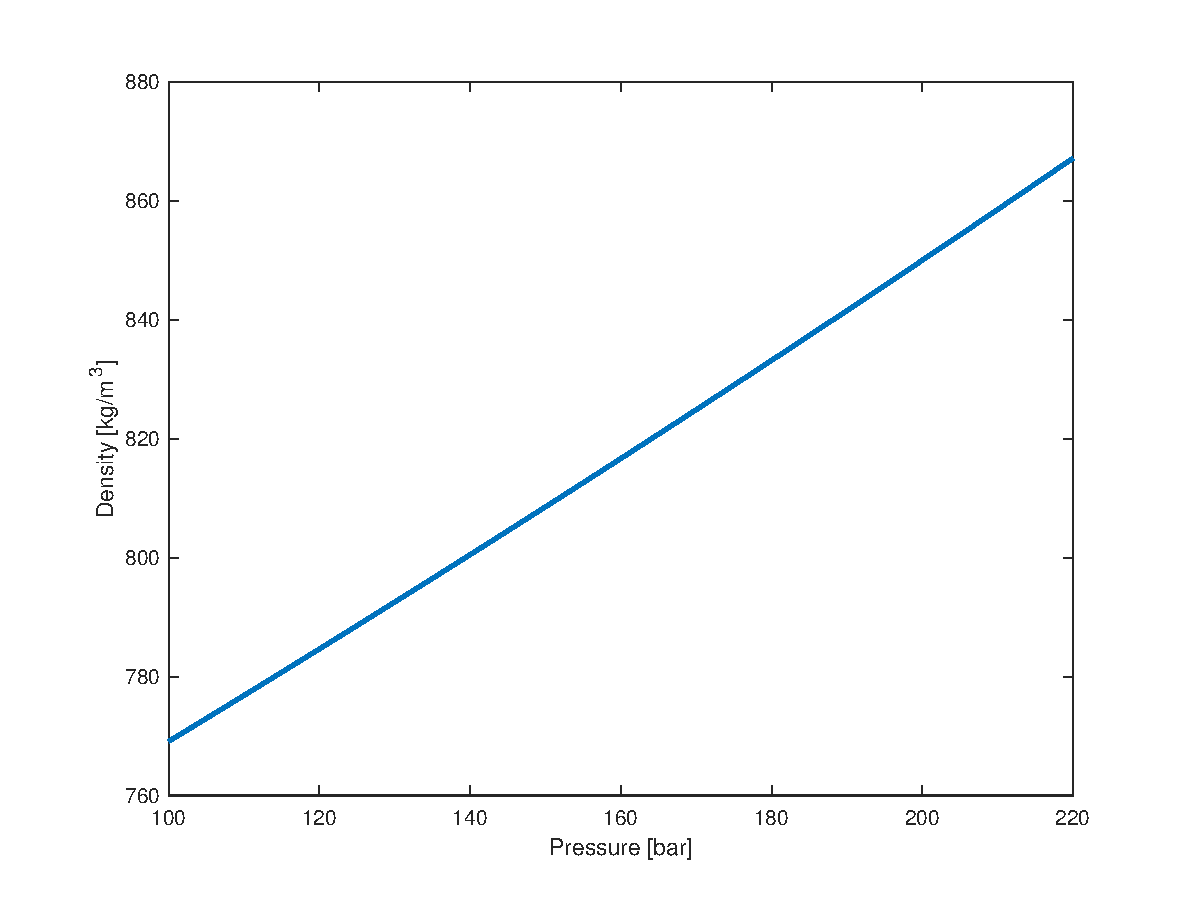
\includegraphics[width=\textwidth]{figures/flow_solver_density.eps}
        \caption{The density of the oil in the reservoir plotted as a function of pressure.}
        \label{fig:flowSolverPoreVolume}
    \end{subfigure}
    \caption{}
\end{figure}

The initial pressure in the reservoir is calculated by solving the nonlinear ODE
\begin{equation*}
    \frac{dp}{dz} = g\cdot \rho(p), \quad p(z = 0) = p_r = 200\text{bar} 
\end{equation*}  
for the fluid density given by Equation \eqref{eq:pressureSolverDensity} and $g$ as the gravity. The well is then inserted by removing 8 grid elements using the \texttt{W = addWell(...)} function. The grid with initial pressure and well can be seen in \autoref{fig:flowSolverGridWithWell}.
\begin{figure}[H]
    \centering
    \begin{subfigure}[t]{0.48\textwidth}
        \centering
        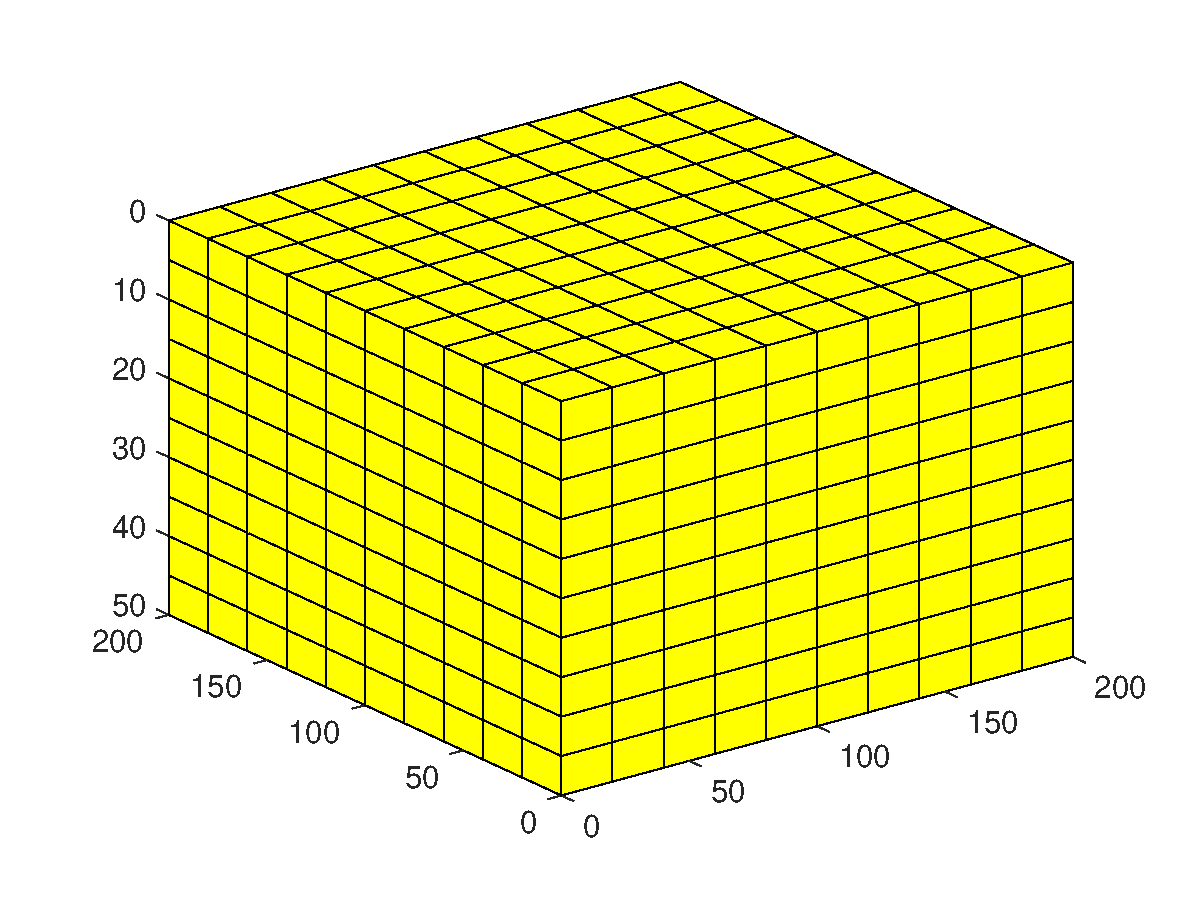
\includegraphics[width = \textwidth]{figures/flowSolver_grid.eps}
        \caption{Uniform $10\times 10 \times 10$ grid of the $200\times 200 \times 50 \text{m}^3$ big reservoir.}
        \label{fig:flowSolverGrid}
    \end{subfigure}
    \hfill
    \begin{subfigure}[t]{0.48\textwidth}
        \centering
        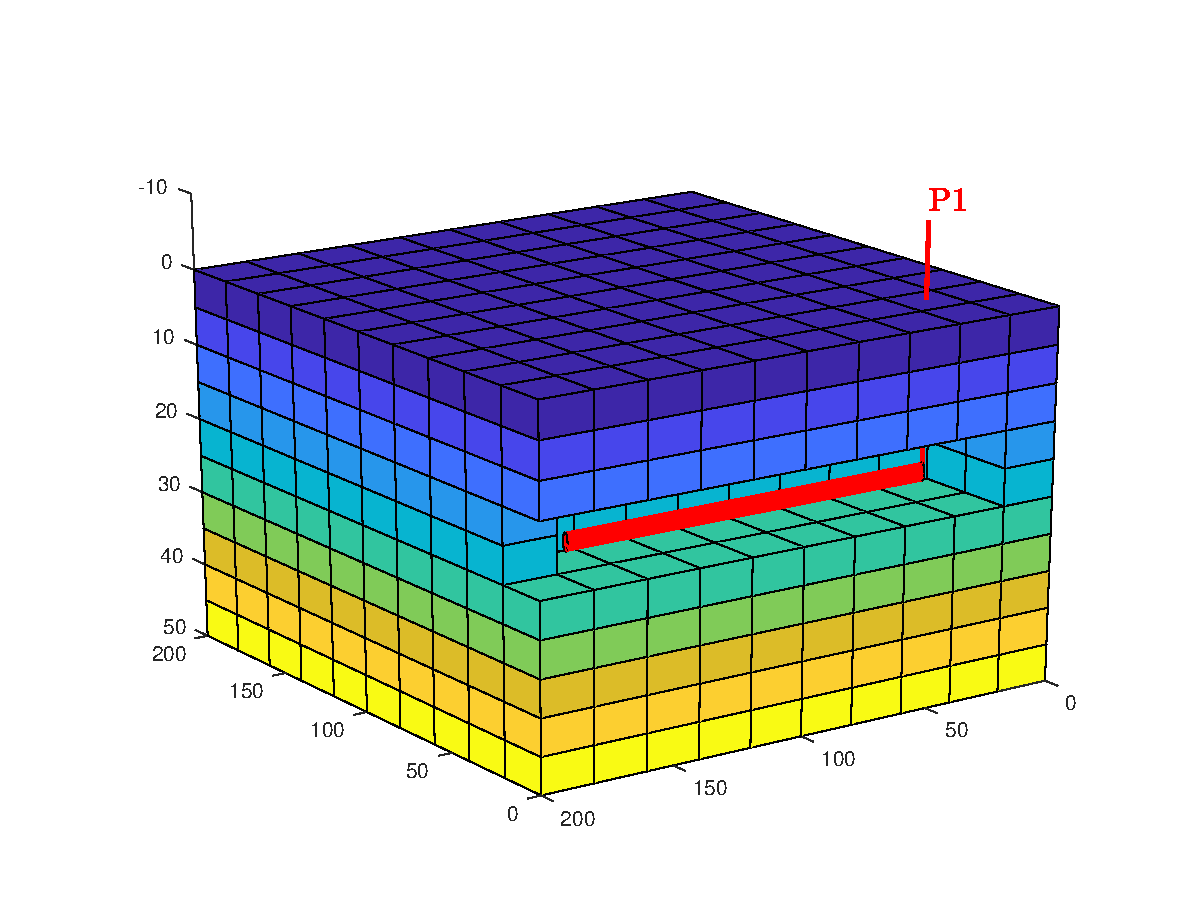
\includegraphics[width = \textwidth]{figures/flowSolver_gridWithWell.eps}
        \caption{Reservoir grid plotted with initial pressure and well P1. Pressure is given in bar. The well has replaced 8 grid elements. Some grid elements are removed to give a better visualization of the well.}
        \label{fig:flowSolverGridWithWell}
    \end{subfigure}
    \caption{}
\end{figure}

\section{Setup of Governing Equations}
After initializing the grid we want to define the discrete gradient and divergence operators, as well as the transmissibilities as explained in Equation \eqref{eq:transmissibility}. This is done by exploiting that we have all the necessary information about the grid properties, such as the cells centroid coordinates, facets areas and so on, stored in the struct \texttt{G}. In \texttt{rock} we have stored the permeability inside each cell that will affect the flux through each facet. With all this information we can now obtain the transmissibilities \texttt{T} and the discrete operators
\lstinputlisting{code/grad_and_div.jl}

The matrix C in the discrete operators are created such that when it is multiplied by the pressure $p$, the result becomes the pressure difference between two adjacent cells, as defined in Equation \eqref{eq:discreteGradient}. The matrix C is stored as a sparse matrix, and the reason why is clear from \autoref{fig:discreteOperatorsC}, which shows the sparse  structure of C. The divergence operator is made using the fact that in the continuous case, the gradient operator is the adjoint of the divergence operator
\begin{equation*}
    \int_\Omega p\nabla \cdot \vec{v} d\Omega + \int_\Omega \vec{v}\nabla p d\Omega = 0.
\end{equation*}
This holds for the discrete case as well \emph{\citep{lieMrstUrl}}, and hence the adjoint of \texttt{C} is the negative transpose of \texttt{C}.

\begin{wrapfigure}{r}{5.5cm}
    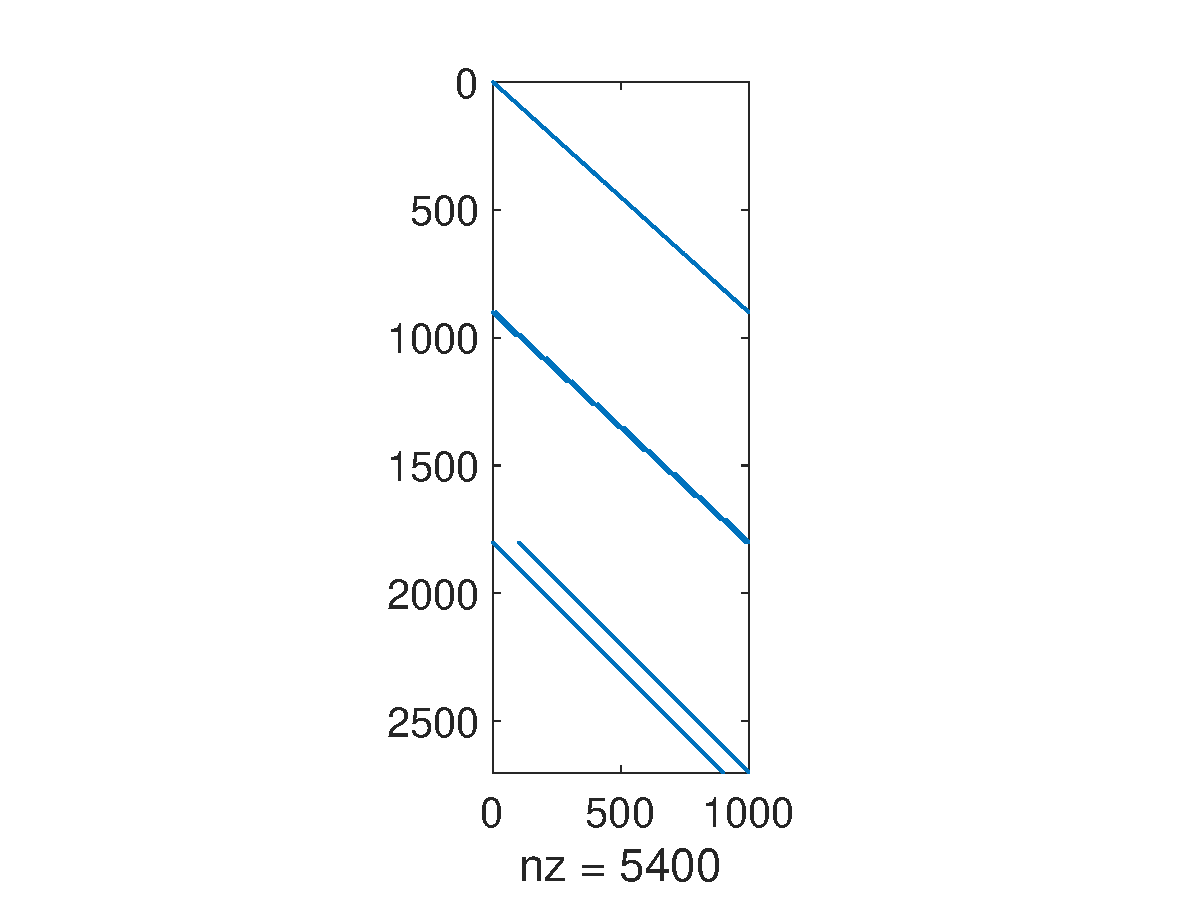
\includegraphics[width=\linewidth]{figures/flowSolver_discrete_operators_C.eps}
    \caption{Structure of discrete operator \texttt{C}.}
    \label{fig:discreteOperatorsC}
\end{wrapfigure}
Now we have all the ingredients to set up the governing equations for the flow in the reservoir. We use a finite volume method to discretize in space, as explained in \autoref{sec:ApplicationsAD}, and a backward Euler method to discretize in time. In the end, all the equations we want to solve should be on residual form, $\boldsymbol{F}(\boldsymbol{x}) = 0$, so that we can use the Newton-Raphson method described in Equation \eqref{eq:newtonRaphsonVector} to solve the system. As there are multiple equations that will be a part of the residual function $\boldsymbol{F}(\boldsymbol{x})$, we define them separately first. One of the advantages of defining the discrete gradient- and divergence operator is that the continuous and discrete forms of the equations look very similar. Hence I will first state the continuous version of the equation and then the discrete, so that it is easy to see how similar they look. I start by defining Darcy's law, which explains how the oil will flow through the porous rock

\begin{equation*}
    \textbf{v} = - \frac{k}{\mu}(\nabla p - \textbf{g}\rho).
    \label{eq:pressSolverDarcy}
\end{equation*}
$k$ is the permeability that we have saved in the \texttt{rock} variable and $\mu$ is the viscosity of the oil.
The corresponding discrete equation that we call \texttt{flux} is given by 
\lstinputlisting{code/flux.jl}
Here, T is the transmissibilities that contain $k$ and the properties of the grid. Since two adjacent cells can have different values of $\rho$, we use the  average for the two cells. \texttt{gradz} is the gradient of the cell centroid's $z$-value. This determines how much the flux depend on $g$ given the orientation of the adjacent cells. When \texttt{flux} is defined, we define the continuity equation in the continuous case
\begin{equation*}
    \frac{\partial}{\partial t}(\phi\rho)(p) + \nabla\cdot(\rho\textbf{v}) = q,
\end{equation*}
where $\phi$ is the porosity of the rock. Since we will handle the well later, the source term $q$ representing injection or production fluids, is set to zero for now. In the corresponding discrete case we get the function
\lstinputlisting{code/presEq.jl}
where \texttt{pv} is the pore volume of the rock given in Equation \eqref{eq:poreVolume} and $p0$ is the pressure at the previous time step. 

In addition, we need a few equations to represent the flow inside the wellbore. This flow will be the production term $q$ we ignored in the derivation of the \texttt{presEq} function. The standard model is to assume that the pressure is in hydrostatic equilibrium inside the wellbore, so that the pressure in a perforated cell (i.e., a cell in which the wellbore is open to the reservoir rock and the fluid can flow in or out of the well) is given as a hydrostatic difference from the pressure at a datum point (the bottom-hole pressure), typically given at the top of the reservoir. That is, the pressure in a perforated cell $c$ is given by
\begin{equation*}
p_c = p_{bh} + g (z_c - z_{bhp})\rho.    
\end{equation*}
In the discrete case this is given by the function \texttt{p\_conn}
\lstinputlisting{code/p_conn.jl}
The pressure drop near the well usually takes place on a much shorter length scale than the size of a grid cell, and is usually modelled through a semi-analytical expression that relates flow rate to the difference between the reservoir and wellbore pressures. Hence the analytic expression for the production in a perforated cell is given by
\begin{equation*}
    q = \frac{\rho}{\mu}\mbox{WI}(p_c - p_r),
\end{equation*}
where \mbox{WI} is the properties of the rock and the oil at the applicable cell. Since this equation only apply on a few of the cells in the reservoir, we also need a list of the indices \texttt{wc} for the perforated cells. These indices and the \mbox{WI} variable are given by the \texttt{W} variable we received from the \texttt{addWell} function. The discrete expression for the production in all the perforated cells are given by
\lstinputlisting{code/q_conn.jl}
The residual expression for the total production \texttt{qS} is then given by summing up all the production from each perforated cell, giving the expression \texttt{rateEq}
\lstinputlisting{code/rateEq.jl}
Here \texttt{rhoS} is the density of the oil at the surface, to obtain the total volume produced. To control the well, we can either set total inflow or outflow of the well (evaluated at surface pressure) to be constant, or set the datum (bottom-hole) pressure as constant. In either case, we will wish to compute the other (i.e., if pressure is given, we determine the surface rate, and vice versa). Herein, we assume pressure to be given as 100 bar and we get
\lstinputlisting{code/ctrlEq.jl}
When all the governing equations are defined, we merge them into one large residual vector function $\boldsymbol{F}(\boldsymbol{x})$. The first 1000 residual equations are the \texttt{presEq} with negative production \texttt{q\_conn} for the indices \texttt{wc}. Equation number 1001 is the \texttt{rateEq} and Equation 1002 is the \texttt{ctrlEq}. Hence, $\boldsymbol{x}\in\Re^{1002}$, where the first 1000 elements are the average pressure in each cell, element 1001 will be the pressure at the datum point inside the well (\texttt{bhp}), and element 1002 is the surface fluid rate \texttt{qS}. Now, if we start by defining \texttt{p}, \texttt{bhp} and \texttt{qS} as AD-variables, $\boldsymbol{F}$ will also be an AD-variable and we will have the Jacobian of the residual vector function $\boldsymbol{F}$. This means we can solve the equations using the Newton-Raphson method, defined in Equation \eqref{eq:newtonRaphsonVector}. A pseudo code of how we solve the system can be seen below.
\newpage
\lstinputlisting{code/press_solver_main_loop.jl}

\section{Flow Solver Results}
If we simulate how the pressure in the reservoir will decay during one year, we will get the result displayed in \autoref{fig:flowSolverResult}.
\begin{figure}[H]
    \centering
    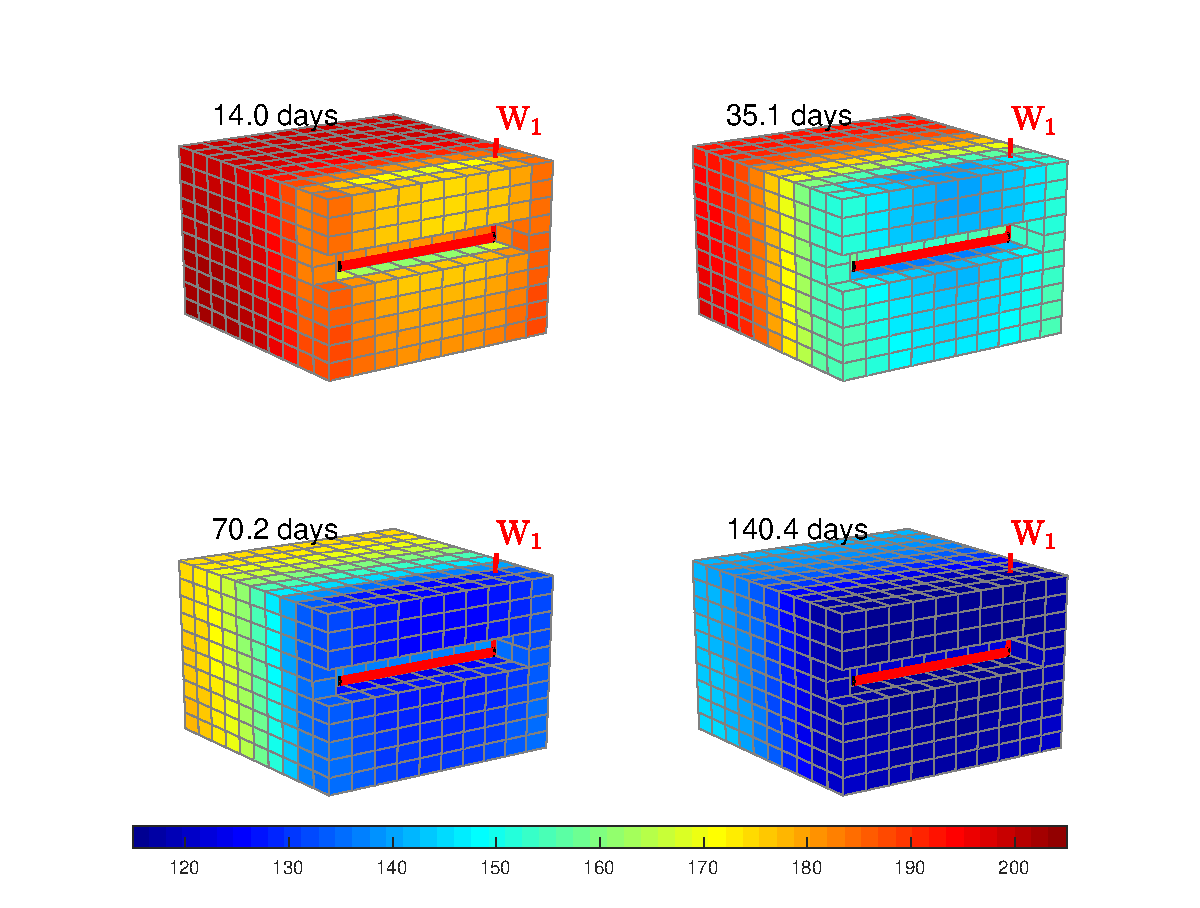
\includegraphics[width = 0.9\textwidth]{figures/flowSolver_result.eps}
    \caption{The pressure in the reservoir displayed at four different times. Pressure is given in bar.}
    \label{fig:flowSolverResult}
\end{figure}
Note the different intervals for the color bar in \autoref{fig:flowSolverResult} compared to \autoref{fig:flowSolverGridWithWell}. With the current color bar interval, at initial state, the whole reservoir will be displayed red. Hence, we can see how the reservoir from the beginning being approximately 200 bar everywhere, begins with the largest pressure decay close to the well, but after some time, the oil is pushed towards the well by the pressure differences and the pressure begins to decay also furthest away from the well. 

\autoref{fig:flowSolverProduction} shows the development of the production rate and the average pressure inside the reservoir. We can see how the production rate follows the average pressure inside the reservoir, and that after some time it approaches zero. This phase is what is called primary production. In primary production, the pressure in the reservoir is so high that there is no need to pump the oil out, the pressure difference does all the work. After some time, we can see that the pressure becomes too low and the production decreases. When this happens, we transit to what is called secondary production. To retrieve more oil from the reservoir we need to apply extra pressure inside the reservoir. This can for example consist of injecting water or gas into the reservoir. This is called the secondary production. More details about how this work can be found in \emph{\cite{lieMrstUrl}}, but the main idea here is that in order to keep up the production and fully exploit the resources in the reservoir, we need to apply external pressure. To do this in the best possible way, it is important to be able to simulate how the pressure evolves inside the reservoir so that we can make good decisions on which actions produce the best possible results. This flow solver is a simple example of how we can model such evolution of the pressure in a reservoir elegantly with governing equations on residual form, created by discrete differentiation operators, and AD.
\begin{figure}[H]
    \centering
    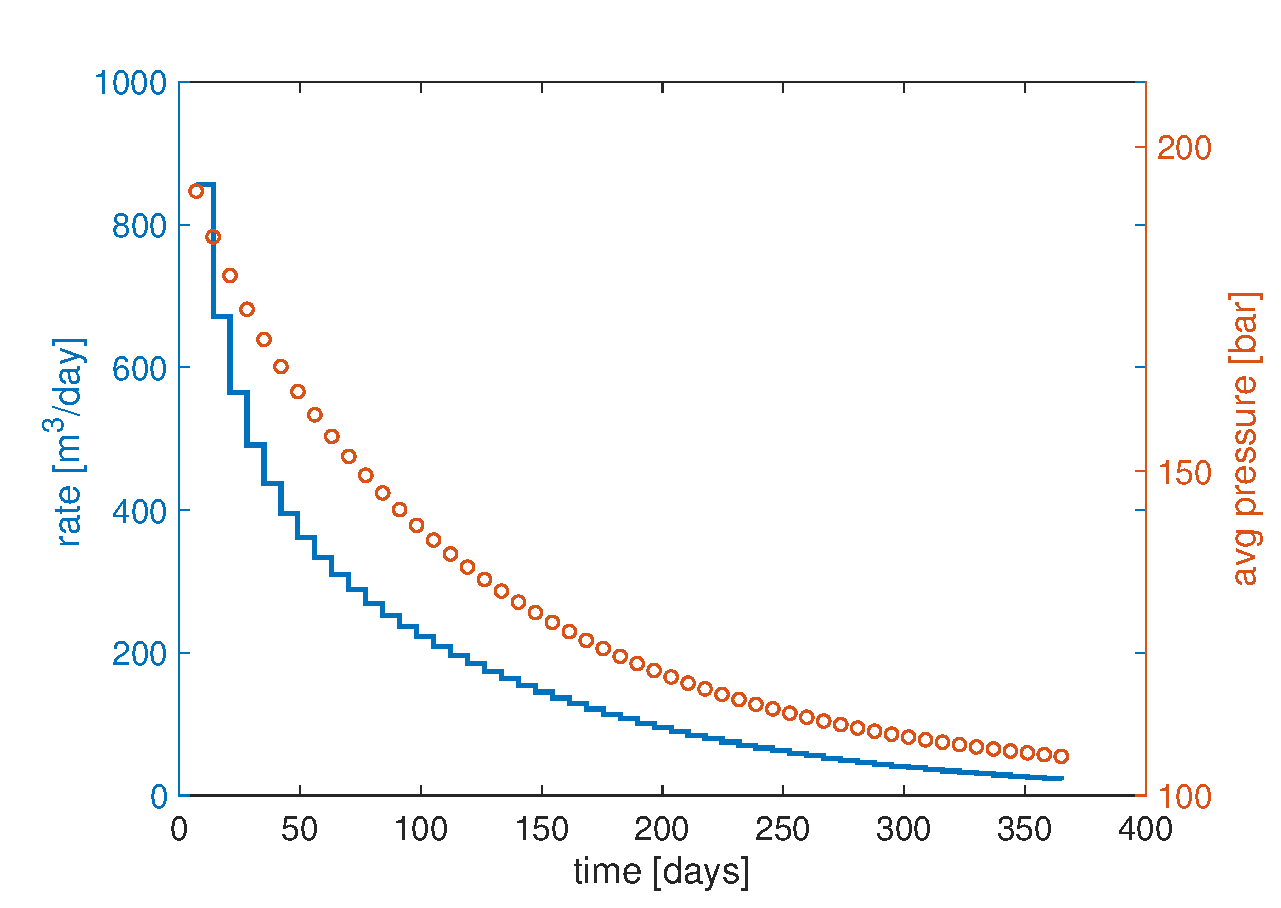
\includegraphics[width = 0.9\textwidth]{figures/flow_solver_production.eps}
    \caption{The production rate and the average pressure in the reservoir as a function of time.}
    \label{fig:flowSolverProduction}
\end{figure}

When it comes to solving the residual equations with the Newton-Raphson method, it is interesting to have a look at how the Jacobian of $\boldsymbol{F}$ looks like. \autoref{fig:flowSolverJacobian} shows the structure of the Jacobian. The first impression is that the matrix is very sparse. Except from a few nonzero points in row 1001 and column 1001 because of the well, the Jacobian consist of 7 diagonals with nonzero elements and the rest of the elements being 0. As there are only 6419 non-zero elements out of more than 1 million matrix elements, it is clear that storing the full $1002\times 1002$ matrix will be very inefficient.

As explained in \autoref{sec:ApplicationsAD}, the different types of AD mentioned store the Jacobians differently. In  \textit{ForwardAutoDiff} and MRST's implementations of AD, the Jacobians are stored as a list of sparse matrices where each Jacobian element in the list is the Jacobian with respect to one primary variable. In this example, this is a lot more efficient than storing the full $1002\times 1002$ Jacobian as  \textit{ForwardDiff} does.
\begin{figure}[H]
    \centering
    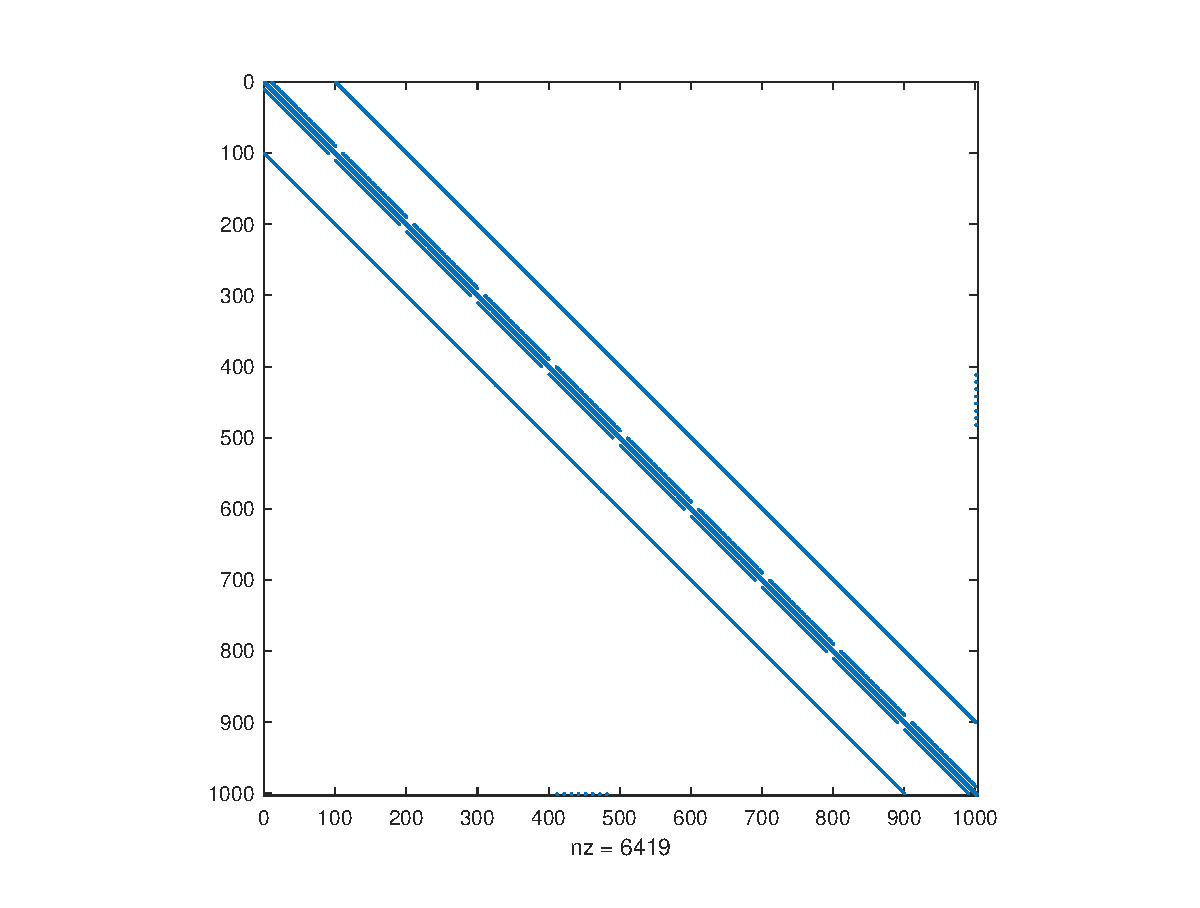
\includegraphics[width = 0.9\textwidth]{figures/flowSolver_Jacobian.eps}
    \caption{Structure of the $1002\times 1002$ Jacobian of the governing equations. There are 6419 non-zero elements.}
    \label{fig:flowSolverJacobian}
\end{figure}

The difference in implementation of the Jacobian should make a big impact on the computation time for this problem. To benchmark the different methods, we need to do some extra work to make sure that it is actually the AD we benchmark and not other parts of the code. This is especially important for the code running in Julia, since when we call MATLAB from Julia it will be a lot of overhead. This means that the setup of the discrete gradient and divergence operators will take longer when done in MATLAB called from Julia, than when we do it directly in MATLAB. If we want to run the full simulation it is not possible to separate the AD part fully, but if we only benchmark the main-loop containing the Newton-Raphson method, AD will be a dominating part of the computations together with the linear solver \texttt{f.jac\textbackslash f.val}. This means we at least will get an indication of how well the AD tools perform compared to each other. To see how the different methods scale as the discretization becomes finer and the system we solve grow, I have benchmarked three different discretizations. The first is the original setup with 10 cells in spatial direction $x$, $y$, and $z$. This gives a total number of 1000 cells in the reservoir. Then, I have also tested the implementations for 20 and 30 cells in the spatial directions. The time spent solving the system for the different methods can be seen in \autoref{tab:FlowSolverSpeedTest}.
\begin{table}[H]
    \centering
    \caption{Table with speed benchmarks of different AD methods solving the "Single-Phase Compressible AD Solver" for different discretizations.}
    \label{tab:FlowSolverSpeedTest}
    \def\arraystretch{1.5}
    \begin{tabular}{ccccc}
    \textbf{Number of cells} & \textbf{ForwardDiff} & \textbf{ForwardAutoDiff} & \textbf{MRST} & $\frac{\textbf{ForwardAutoDiff}}{\textbf{MRST}}$\\
        \hline
         $10\times10\times10$ & 71.5s & 2.3s & 1.9s & 1.21 \\  
         $20\times20\times20$ & ~ & 31.9s & 23.4s & 1.36\\ 
         $30\times30\times30$ & ~ & 188.8s & 147.8s & 1.28\\ \hline
    \end{tabular}
\end{table}
For 10 cells in each spatial direction it is clear that what I assumed based on the structure of the Jacobian in \autoref{fig:flowSolverJacobian} is true; The  \textit{ForwardDiff} method takes much longer time than  \textit{ForwardAutoDiff} and MRST. Since  \textit{ForwardDiff} already spends over a minute for $10\times 10\times 10$ cells, it is omitted for finer discretizations. According to the results in \autoref{tab:FlowSolverSpeedTest}, MRST is a bit faster than  \textit{ForwardAutoDiff}. We can also see from the column farthest to the right that the ratio between time spent using MRST and  \textit{ForwardAutoDiff} stays approximately constant as the complexity of the problem grows. This indicates that the two different solvers scales equally. It is, although, not possible to say if it is the AD or the linear solver part that makes the solver in MATLAB faster than the one in Julia. To get a better indication of what part of the code makes the difference, I have tested the speed of the linear solvers solving the system \textbf{Ax} = \textbf{b} in MATLAB and Julia. The built in linear solvers use different methods based on the structure of the matrix. Hence, to make the test as relevant as possible, I have used the Jacobian from the first step of the flow solver as the matrix \textbf{A}. The \textbf{b} vector is a randomized vector of values between 0 and 1. The results for the three different discretizations with 10, 20 and 30 cells in each spatial direction can be seen in \autoref{fig:benchmarkLinearSolver}. 
\begin{figure}[H]
    \centering
    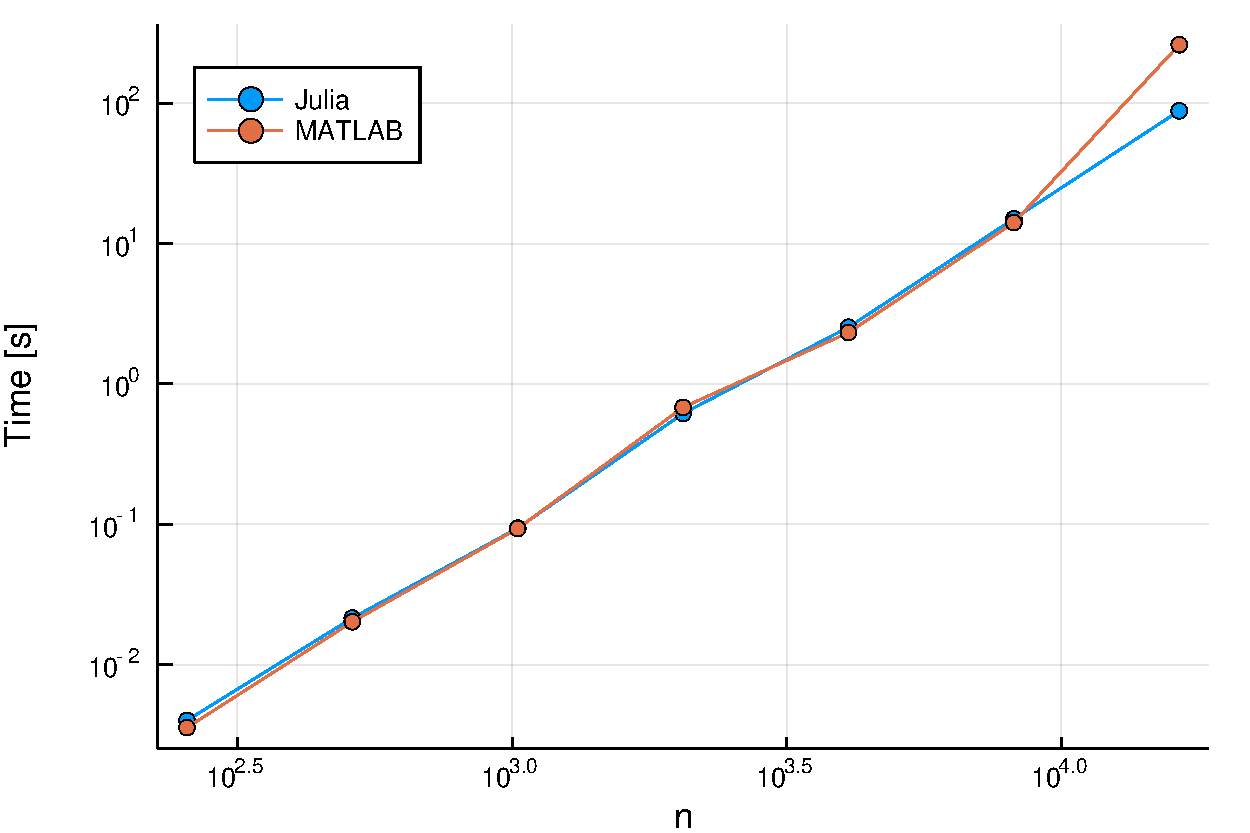
\includegraphics[width = 0.9\textwidth]{figures/benchmark_linear_solvers.pdf}
    \caption{Computational time for solving the system \textbf{Ax} = \textbf{b} for \textbf{x}$\in\Re^{n}$ and \textbf{A} = \textbf{J}, the Jacobian from the first step in the flow solver.}
    \label{fig:benchmarkLinearSolver}
\end{figure}
We can see that the linear solvers perform very similar for all three cases, with MATLAB having small victories in computation time for 10 and 20 cells and Julia for 30. With this in mind, we can say that the linear solvers in MATLAB and Julia perform so similar that it is a valid assumption to assume that they perform equally well. Hence the speed differences in \autoref{tab:FlowSolverSpeedTest} is most likely because of speed differences in the AD-tools. This means that for the equations in the "Single-phase Compressible AD Solver" example, the \textit{ForwardAutoDiff} implementation is approximately 30\% slower than the AD tool in MRST.